\subsection{UNET embeddings}
    \label{section:unet-embeddings-study}
    As well as one autoencoder embeddings that represent a high-dimensional input in lower dimensional space, UNet embeddings provide useful and interesting information on the predictions quality. However, it is important to keep in mind that the dimensionality of embeddings in the UNet case is not lower than the dimensionality of the input and is even often higher (see the UNet architecture in Figure \ref{fig:unet}). The goal of a UNet in contrast to an autoencoder is not to compress the input, but to extract useful features that are helpful for high-resolution segmentation. UNet embeddings do not contain rich image semantics in them as the embeddings of an autoencoder do. UNet compresses the spatial dimension of the input, but at the sme time it gradually increases the number of filters that capture of information need for segmentation. As has been proven in Section \ref{section:nuclei-predictions} having more filters only helps to get better predictions, therefore there is no need for a UNet to have low-dimensional embeddings. Nevertheless, it is still interesting to see if the embeddings do contain any information about the input that one could use. There were two hypotheses put in question: the first one is whether embeddings of a trained UNet form any kind of clusters based on a cell's phenotype. The second hypothesis is whether embeddings of corrupted images can be clustered together further away from non-corrupted ones. If the latter hypothesis would hold true, one could alarm the end user about the outliers in the dataset based on their distance from both of the clusters. 
    \subsubsection{Application of various dimensionality reduction methods}
        \label{section:unet-embeddings-dim-reduction}
        \begin{figure}[H]
	\begin{center}
		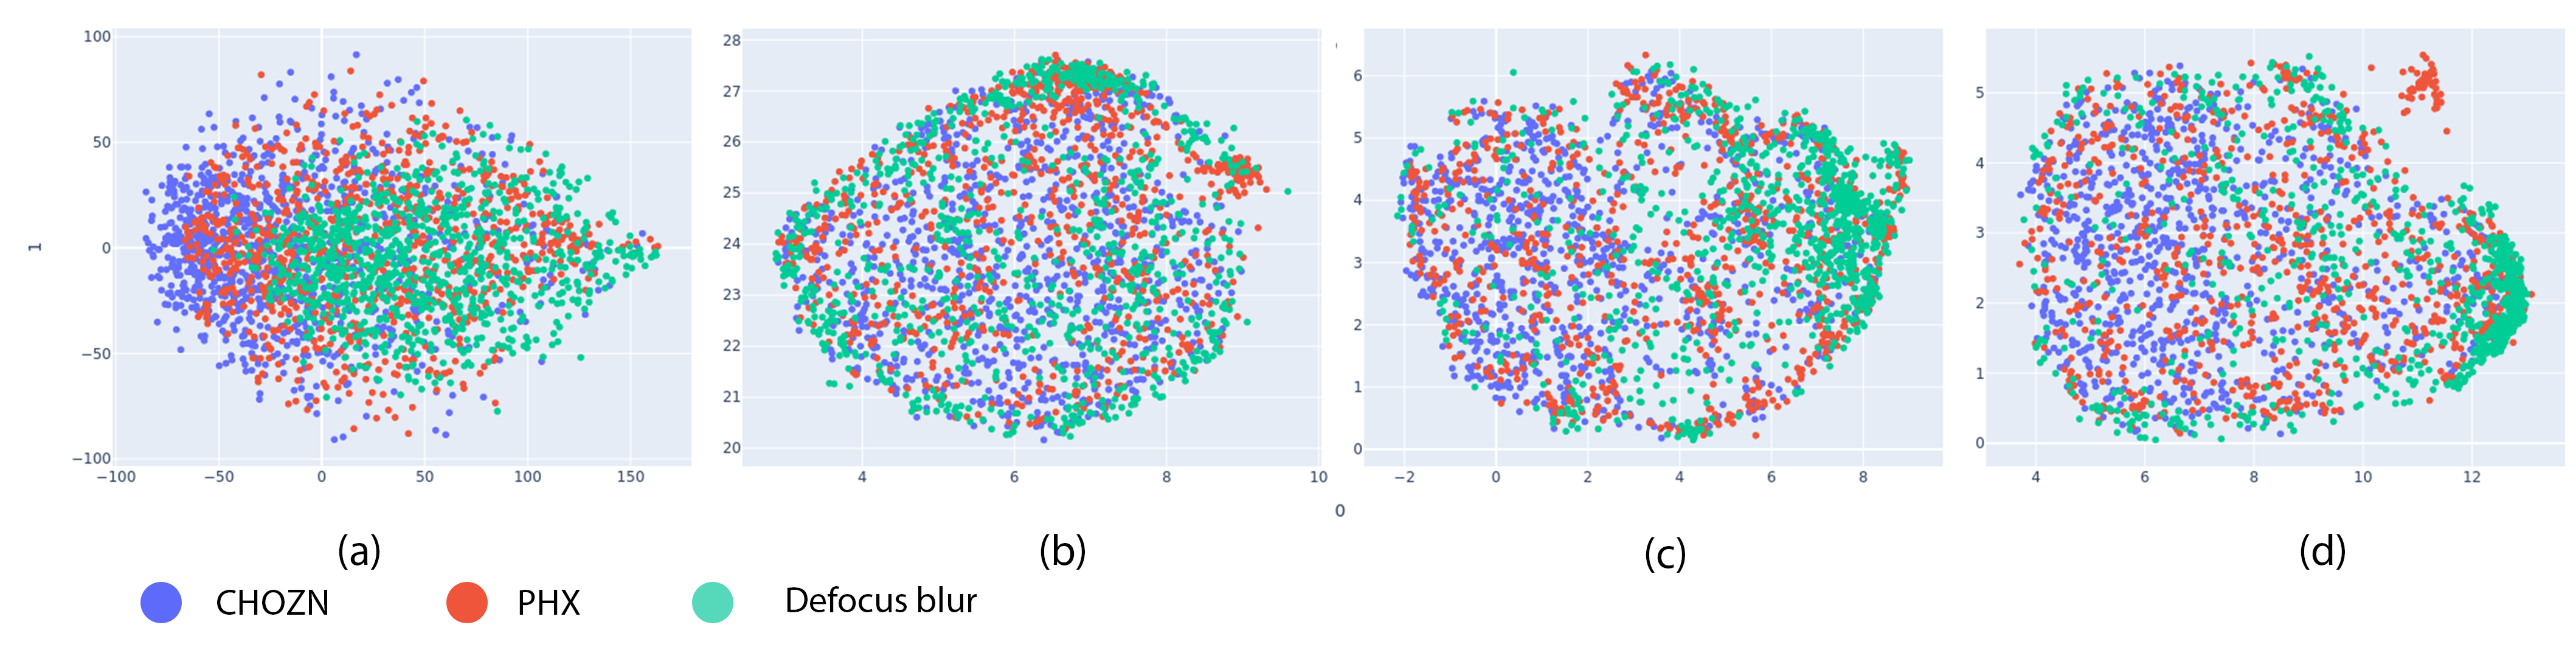
\includegraphics[width=\linewidth]{bilder/unet-embeddings/umap-pca-embeddings.png}
		\caption{(a) PCA, (b) UMAP, (c) combination of PCA and UMAP with 10 and (d) 50 components}\label{fig:umap-pca-embeddings}
	\end{center}
\end{figure}

    \subsubsection{Autoencoder embeddings as an alternative}
        Since UNet embeddings do not seem to exhibit any exceptional results in terms of clustering, it was decided to train an autoencoder directly on DIC image crops. Since the autoencoder's embeddings contain dense semantic information of the input they might provide more insights for clustering the previously mentioned hypotheses. Figure \ref{fig:ae-training} presents the architecture of two convolutional autoencoders used for these experiments. One compresses $256 \times 256$ input crops into embeddings vector of size $3528$ and another one compresses them into a vector of a smaller size of $200$. Both autoencoders were trained using MSE loss. The results of their convergence are presented in Figure \ref{fig:ae-training} on the right.

\begin{figure}[H]
	\begin{center}
		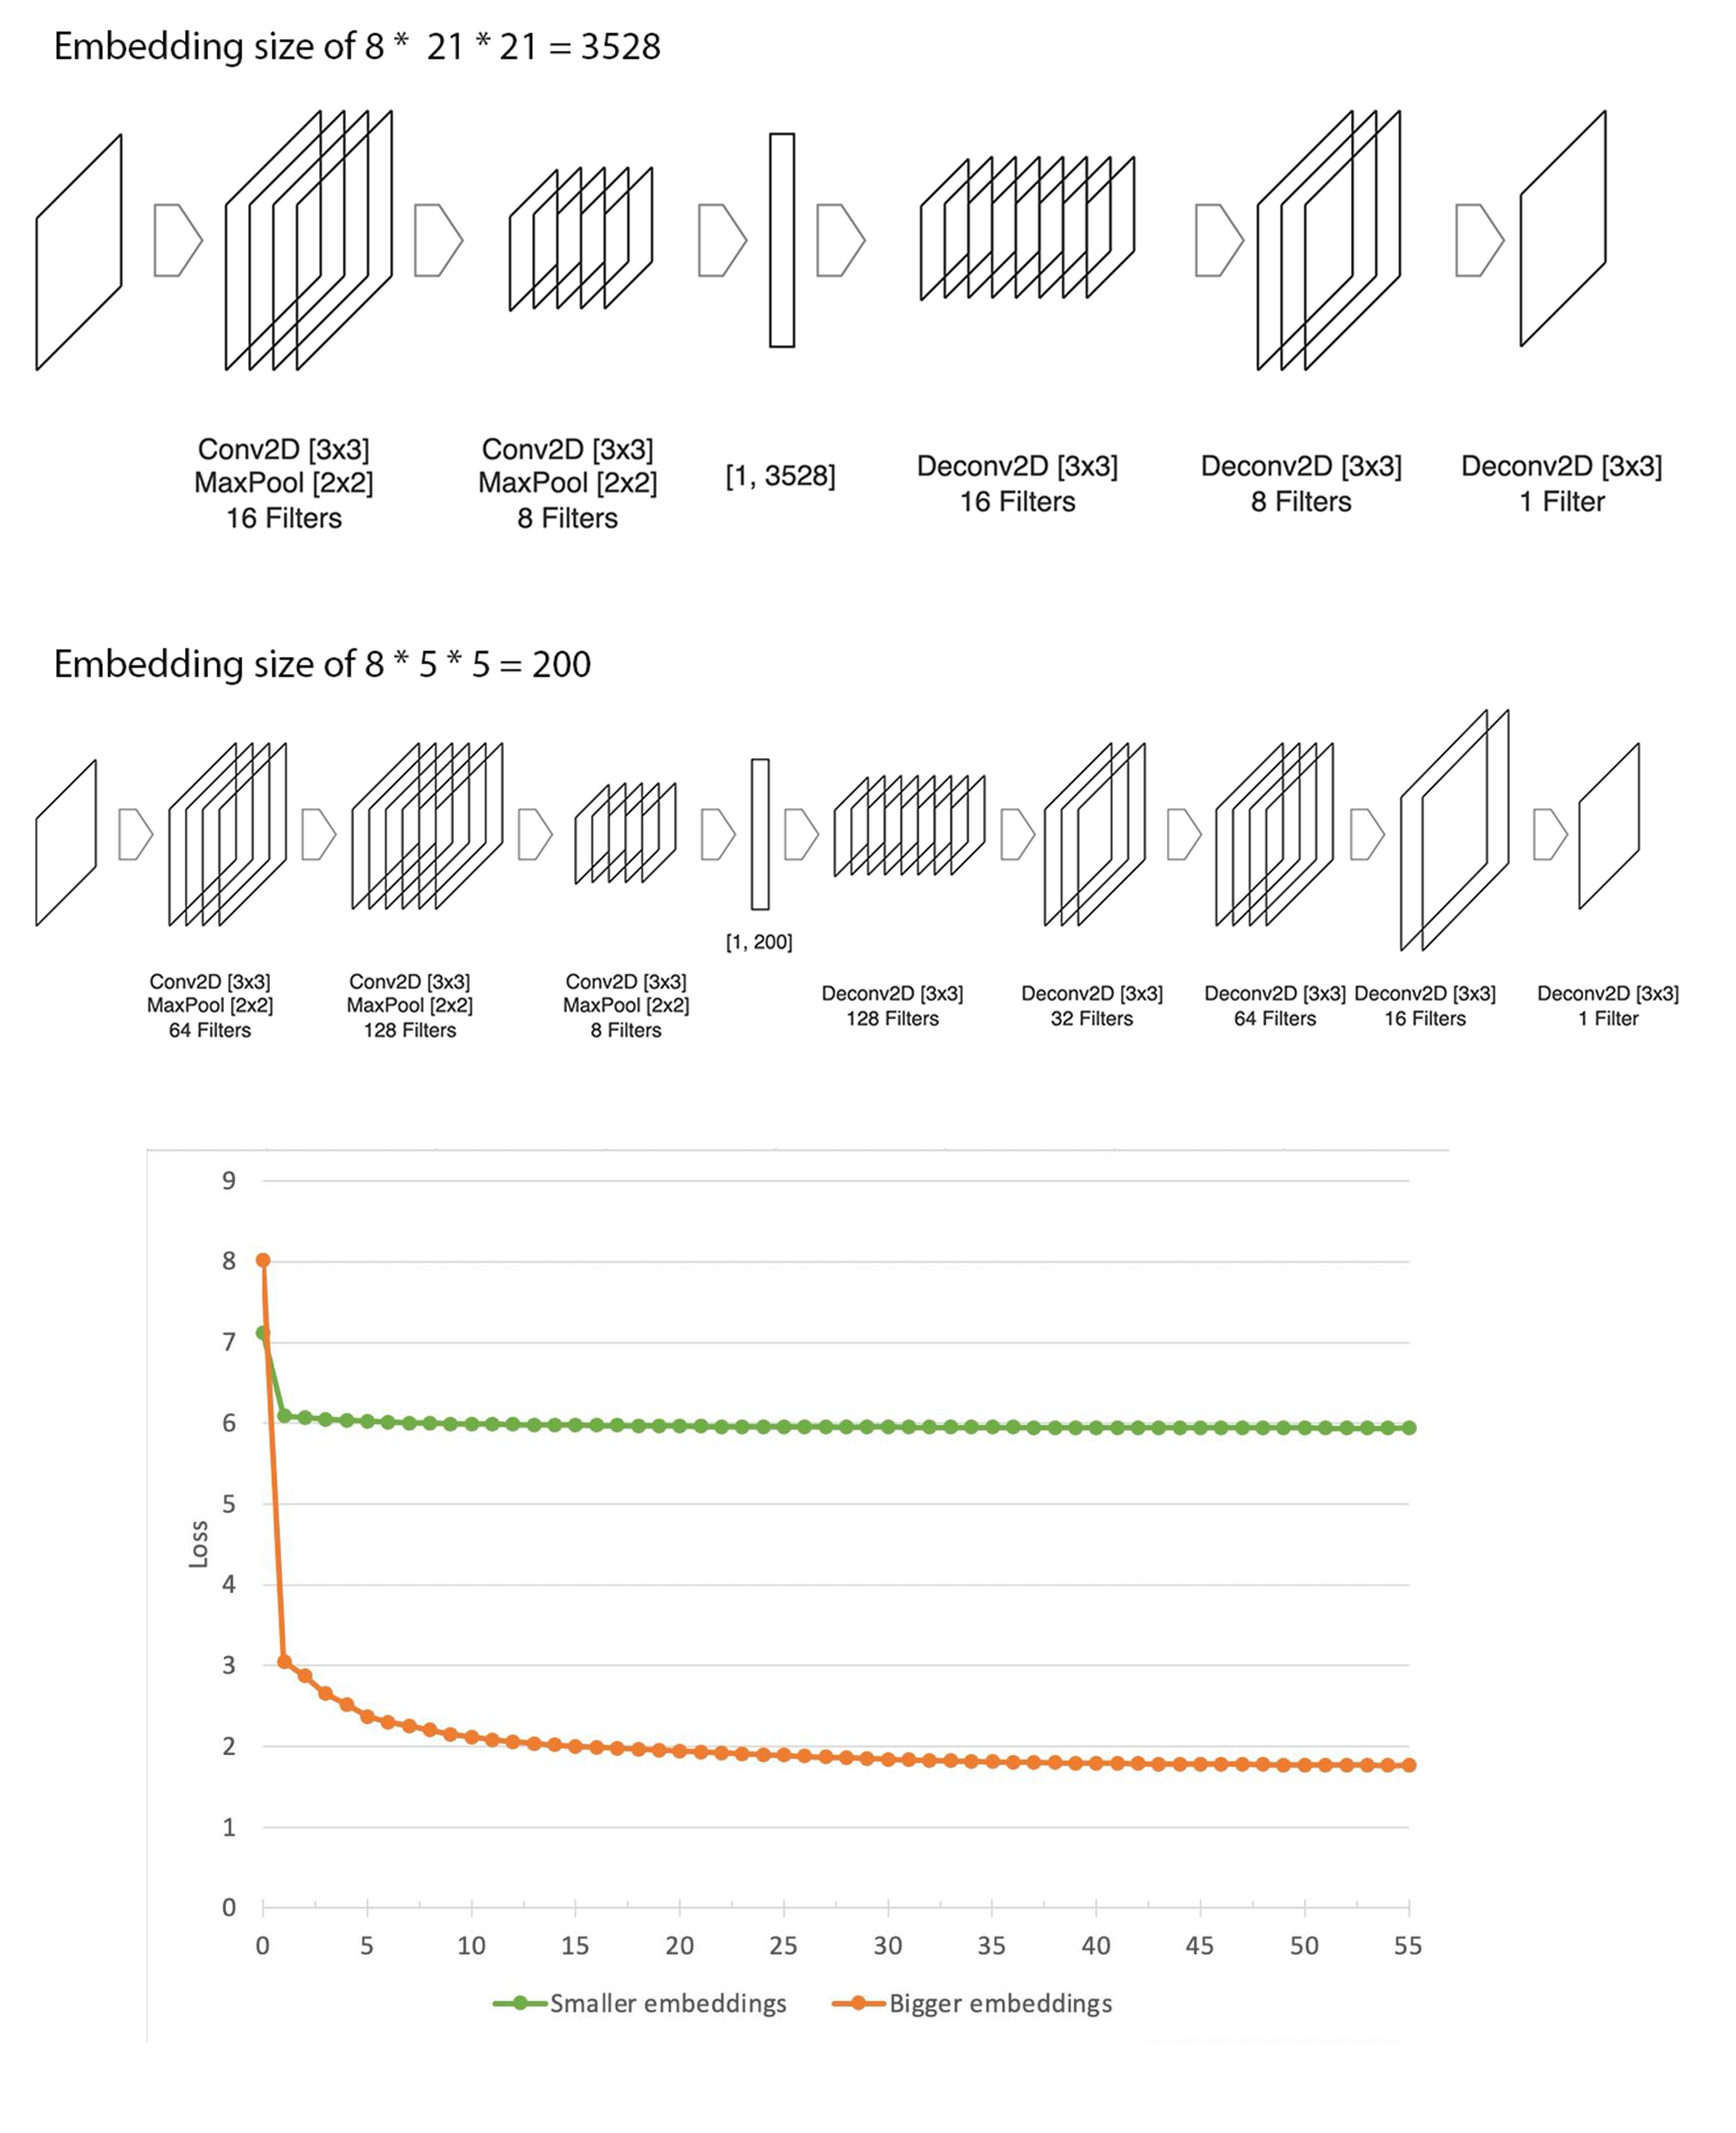
\includegraphics[width=\linewidth]{bilder/ae-embeddings/training-architectures.png}
		\caption{Architectures of two autoencoders and their training convergence}\label{fig:ae-training}
	\end{center}
\end{figure}

An autoencoder with embeddings of bigger size was able to achieve a lower loss as well and the samples reconstructed from it were of higher quality (see Figure \ref{fig:ae-samples}). Clearly reconstruction of the samples will not have a high resolution as there are no skip-connections in this architecture. However, this is also not needed, the main goal here is to find out whether autoencoder embeddings provide any insights on the data.
\begin{figure}[htb]
	\begin{center}
		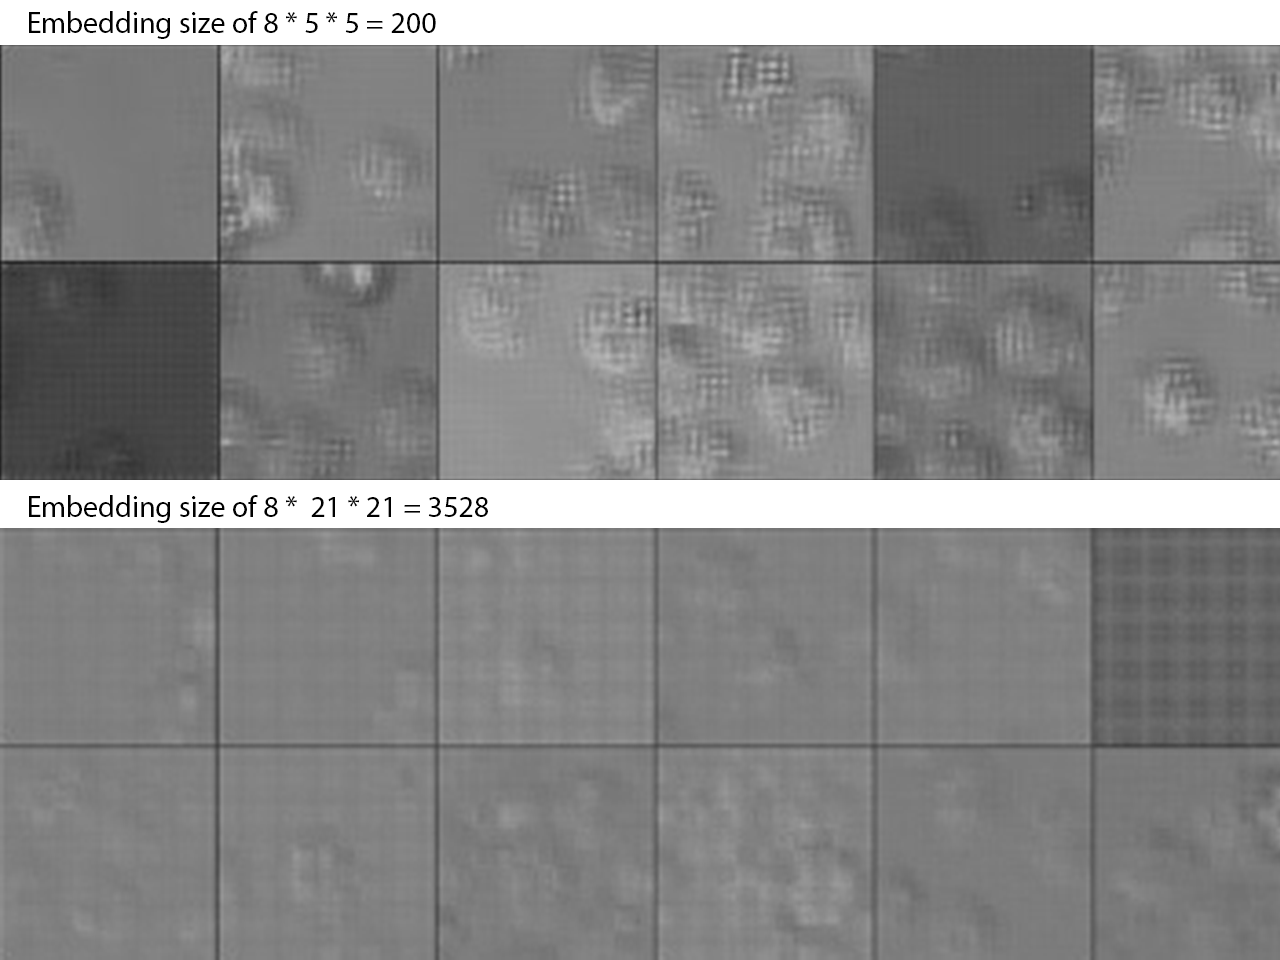
\includegraphics[width=0.5\linewidth]{bilder/ae-embeddings/ae-samples.png}
		\caption{Samples drawn from trained autoencoders. (a) --- an autoencoder with a smaller bottleneck layer, (b) --- an autoencoder with a bigger bottleneck layer}
		\label{fig:ae-samples}
	\end{center}
\end{figure}

Since an autoencoder with bigger embedding size seems to be able to reconstruct crops much better we have proceeded with its architecture. Embeddings were projected into a two-dimensional space using first PCA with 10 components and then applying UMAP on PCA's projections. The results of such projection are presented in Figure \ref{fig:ae-pca-umap-clustered}. Two clearly defined clusters appear: the left plot presents projections from an earlier epoch, the right one from a later one. Embeddings separate gradually into two clusters throughout the training.

\begin{figure}[htb]
	\begin{center}
		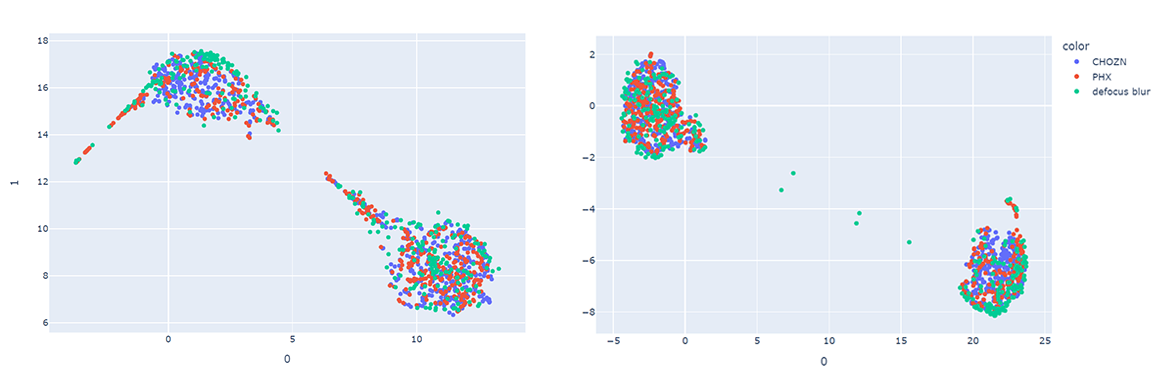
\includegraphics[width=0.5\linewidth]{bilder/ae-embeddings/pca-umap-clusters.png}
		\caption{Autoencoder embeddings after applying PCA and UMAP afterwards}\label{fig:ae-pca-umap-clustered}
	\end{center}
\end{figure}

However, these two clusters are based neither on cell phenotypes nor on input corruption. All points of both phenotype as well as corruptions seem to be equally spread between two clusters. By looking at the images corresponding to each of the clusters it soon becomes apparent that the main difference between them is their brightness level.  To prove this theory distributions of average image intensity of images in both clusters are presented in Figure \ref{fig:ae-brighter-darker}. In the violin plots we can see that the distribution of the crops on the left has a much lower brightness level than the distribution of the crops on the right. However, it is hard to account for why the brightness were different, it might happed due to many different reasons, for example, the images might have been taken on different days when the microscopy lighting conditions might have been different.
%\begin{figure}[htb]
%	\begin{center}
%		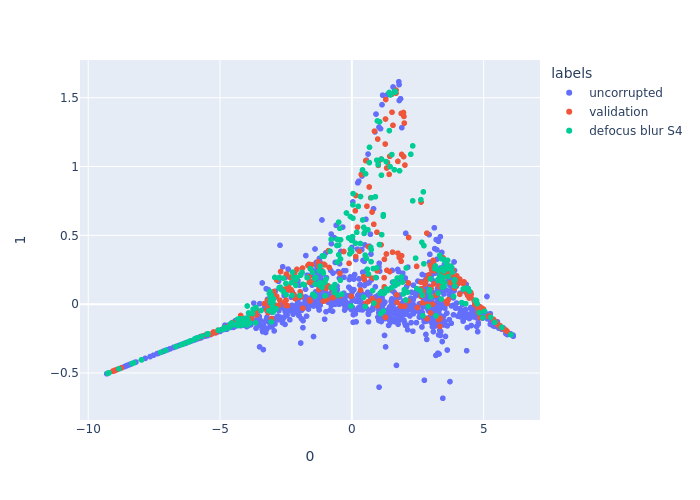
\includegraphics[width=0.5\linewidth]{bilder/ae-embeddings/pacmap.png}
%		\caption{PacMAP does not provide information on the coruption}\label{fig:ae-pacmap}
%	\end{center}
%\end{figure}

\begin{figure}[htb]
	\begin{center}
		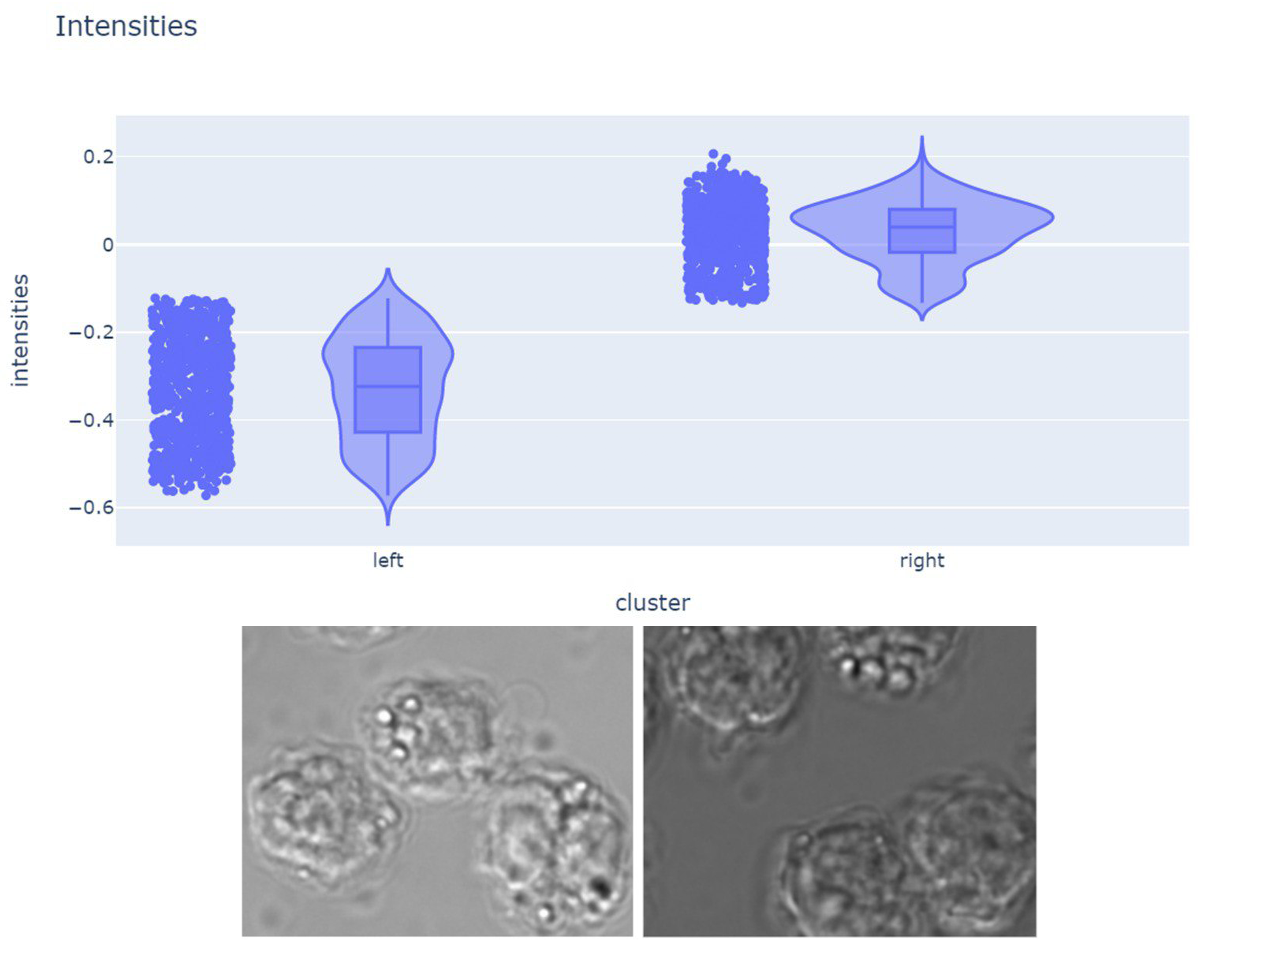
\includegraphics[width=0.5\linewidth]{bilder/ae-embeddings/brighter-darker.png}
		\caption{Different in brightness in the clusters formed by an autoencoder embeddings in a two-dimensional space}
		\label{fig:ae-brighter-darker}
	\end{center}
\end{figure}

Since an autoencoder picks up on brightness difference within the crops, it is worth trying to normalize crop brightness across the entire dataset first. Nevertheless, it is not a trivial task as images have different cell density in them. This is why some images that contain primarily background pixels will always be darker than the ones that contain enough of foreground. We suggest to filter the crops based on the amount of cell criteria (which can be done using GFP model that can detect cells present in DIC) and normalize them afterwards. Retraining the autoencoder with new training data might provide more insights when the difference in brightness is gone.

It is also clear why autoencoder embeddings do not provide any clustering for corrupted crops. Corruption severities neither really change the image semantics nor are they significantly different visually speaking (see defocus blur in \ref{fig:artificial-corruptions}). Therefore they do not alter the ability of an autoencoder to restore input correctly. In contrast, UNet's fluorescence predictions do suffer significantly for several corruption levels, its predictions strongly change --- the outline of organelles becomes more blurry, additional shine appears in fluorescence prediction. These changes happen not only during the decoding part, but they also might bring unsual values in the embedding representation. Therefore UNet embeddings have more information on the "trustworthiness" of predictions. That is why when defocus corruptions are used as training augmentations, drift detection for the model trained with these corruptions stops alarming about the drift. Even though it did for the model, which did not have these augmentations present [TODO add section reference]. This happens simply because the models' predictions degrade and start looking different, which triggers a "drift alarm". With the improved predictions, drift alarm would not be triggered even when using the same data.